\cleardoublepage
\chapter{Descripción informática}

% Descripción del proyecto realizado. Después de unos párrafos introductorios el capítulo se divide en subcapítulos. (de 25 a 35 páginas)

% \section{Requisitos}
% \label{sec:requisitos}

% Descripción detallada de las funcionalidades que tendría que implementar la aplicación (pues se asume que los requisitos se escriben antes de empezar el desarrollo). Pueden tener forma de historias de usuario o bien ser una lista de requisitos funcionales y no funcionales.

% \section{Arquitectura y Análisis}
% \label{sec:arquitectura-analisis}

% Descripción de los aspectos de alto nivel de la aplicación. Diagramas de clases de análisis, diagramas de clases de diseño, etc. Se debe incluir la suficiente información para que el lector pueda entender la estructura de alto nivel del software desarrollado. Se pueden incluir diagramas de casos de uso si se considera útil.

% \section{Diseño e Implementación}
% \label{sec:diseno-implementacion}

% Descripción de algún aspecto relevante de la implementación que quiera mencionarse. Por ejemplo se podría incluir alguno de los siguientes aspectos:
% \begin{itemize}
%   \item Algoritmo complejo que se haya tenido que desarrollar.
%   \item Integración entre librerías problemática.
%   \item Resolución de algún bug que haya sido especialmente problemático.
%   \item Focalizar en alguna parte del desarrollo y describirla en más detalle.
% \end{itemize}

% En esta sección se pueden incluir fragmentos de código fuente. También se pueden incluir algunas métricas del proyecto (número de clases, líneas de código, etc.). También se puede incluir la evolución del repositorio de GitHub (gráfico de commits por día).

% \section{Pruebas}
% \label{sec:pruebas}

% En esta sección se describen las pruebas automáticas que han sido implementadas para el proyecto. Sobre los tests, conviene indicar la cobertura del código. Si no se han implementado pruebas automáticas, deberían haberse implementado y describirse aquí o tener una buena justificación de por qué no se han implementado.


\section{Requisitos}
\label{sec:requisitos}

La aplicación \textbf{Pinche} nace con el objetivo de facilitar la organización de la compra doméstica mediante una aplicación móvil accesible, intuitiva y práctica. Para ello, se han definido una serie de requisitos funcionales que reflejan las necesidades del usuario final, así como requisitos no funcionales que garantizan la calidad de la aplicación.

\subsection{Requisitos funcionales}

Para definir los requisitos funcionales se ha seguido una metodología personalizada que combina las fortalezas de las metodologías \textbf{Scrum}, \textbf{Kanban} y \textbf{Extreme Programming (XP)}. Se ha seguido la estructura iterativa de Scrum, utilizando tableros Kanban para visualizar el flujo de tareas y adoptando buenas prácticas como pruebas continuas e integración frecuente propias de XP.

La organización del desarrollo ha comenzado con la definición de \textbf{historias de usuario}, expresadas en el formato: ``Como [tipo de usuario], quiero [funcionalidad] para [beneficio]''. El esfuerzo y tiempo necesario para implementar estas historias de usuario se ha estimado mediante la técnica de \textbf{Story Points} basada en la sucesión de Fibonacci.

Las historias se han agrupado en \textbf{épicas}, agrupaciones lógicas que organizan funcionalidades principales: \textit{Cuenta de usuario}, \textit{Lista de la compra}, \textit{Recetas} e \textit{Invitados}.

La épica \textit{Cuenta de usuario} agrupa un total de seis historias de usuario con sus respectivas tareas:

\begin{enumerate}
  \item Como usuario, necesito registrarme en la aplicación con la finalidad de poder utilizarla. Estimación: 2 puntos de historia.
  \item Como usuario, necesito iniciar sesión en la aplicación con la finalidad de acceder a mi cuenta de usuario y mis datos. Estimación: 1 punto de historia.
  \item Como usuario, necesito cerrar sesión en la aplicación con la finalidad de no dejar mi cuenta activa en un dispositivo. Estimación: 1 punto de historia.
  \item Como usuario, quiero recuperar mi contraseña de mi cuenta de usuario de la aplicación con la finalidad de poder acceder a mi cuenta. Estimación: 1 punto de historia.
  \item Como usuario, quiero ver un resumen de mi actividad con la finalidad de conocer cuál es mi uso de la aplicación. Estimación: 2 puntos de historia.
  \item Como usuario, necesito eliminar mi cuenta de usuario de la aplicación con la finalidad de borrar mis datos y dejar de tener cuenta de usuario en la aplicación. Estimación: 1 punto de historia.
\end{enumerate}

La épica \textit{Lista de la compra} agrupa un total de trece historias de usuario:

\begin{enumerate}
  \item Como usuario, quiero ver el listado de las listas de la compra que he creado con la finalidad de saber cuántas y qué listas de la compra tengo. Estimación: 2 puntos de historia.
  \item Como usuario, quiero ver el listado de listas de la compra que aún no han sido completadas con la finalidad de poder visualizar más fácilmente que listas tienen artículos por comprar. Estimación: 1 punto de historia.
  \item Como usuario, quiero acceder al detalle de una lista de la compra en concreto con la finalidad de ver sus artículos. Estimación: 1 punto de historia.
  \item Como usuario, quiero eliminar una lista de la compra, aunque haya sido o no completada, con la finalidad de dejar de visualizarla en mi listado. Estimación: 1 punto de historia.
  \item Como usuario, quiero seleccionar como comprados todos los artículos de una lista de la compra con la finalidad de poder completar una lista en un solo click. Estimación: 1 punto de historia.
  \item Como usuario, quiero seleccionar como pendientes de comprar todos los artículos de una lista con la finalidad de volver a reutilizar esa lista. Estimación: 1 punto de historia.
  \item Como usuario, quiero añadir una nueva lista de la compra con la finalidad de tener una nueva lista donde organizar mis artículos. Estimación: 1 punto de historia.
  \item Como usuario, quiero añadir un artículo a una lista de la compra con la finalidad de recordar que tengo que comprar dicho artículo. Estimación: 1 punto de historia.
  \item Como usuario, quiero seleccionar un artículo como comprado con la finalidad de poder visualizar qué artículos ya he comprado. Estimación: 1 punto de historia.
  \item 	Como usuario, quiero seleccionar un artículo que ya había seleccionado como comprado como no comprado en una lista de la compra con la finalidad de poder volver a tener ese artículo como pendiente de comprar. Estimación: 1 punto de historia.
  \item Como usuario, quiero eliminar un artículo de una lista de la compra con la finalidad de dicho artículo deje de formar parte de la lista de la compra. Estimación: 1 punto de historia.
  \item Como usuario, quiero especificar el nombre del artículo, la cantidad, la unidad de medida de esa cantidad, la tienda donde prefiero comprar y opcionalmente una fotografía del artículo, con la finalidad de disponer de toda la información que necesito de ese artículo. Estimación: 2 puntos de historia.
  \item Como usuario, quiero editar la información de un artículo de una lista de la compra con la finalidad de modificar su contenido. Estimación: 1 punto de historia.
\end{enumerate}

La épica \textit{Recetas} agrupa un total de ocho historias de usuario:

\begin{enumerate}
  \item Como usuario, quiero ver un listado con mis recetas con la finalidad de conocer que recetas tengo registradas. Estimación: 2 puntos de historia.
  \item Como usuario, quiero añadir una nueva receta desde la pantalla de listas de recetas con la finalidad de añadir una nueva receta y sus datos. Estimación: 1 punto de historia.
  \item Como usuario, quiero editar una receta con la finalidad de actualizar datos de esa receta. Estimación: 1 punto de historia.
  \item Como usuario, quiero eliminar una receta con la finalidad de que no aparezca esa receta en mi listado de recetas. Estimación: 1 punto de historia.
  \item Como usuario, quiero acceder a la información de una receta desde la pantalla de lista de recetas con la finalidad de ver en detalle los datos de esa receta. Estimación: 1 punto de historia.
  \item Como usuario, quiero añadir información a una nueva receta con la finalidad de tener toda su información recopilada. Estimación: 2 puntos de historia.
  \item Como usuario, quiero editar la información de una receta con la finalidad de tener la información de esa receta actualizada. Estimación: 1 punto de historia.
  \item Como usuario, quiero eliminar una receta con la finalidad de eliminar esa receta de mis recetas. Estimación: 1 punto de historia.
\end{enumerate}

La épica \textit{Invitados}, agrupa un total de ocho historias de usuario:

\begin{enumerate}
  \item Como usuario, quiero ver un listado con mis invitados con la finalidad de conocer que invitados tengo registrados. Estimación: 2 puntos de historia.
  \item Como usuario, quiero añadir un nuevo invitado desde la pantalla de listas de invitados con la finalidad de añadir un nuevo invitado y sus datos. Estimación: 1 punto de historia.
  \item Como usuario, quiero editar un invitado con la finalidad de actualizar datos de ese invitado. Estimación: 1 punto de historia.
  \item Como usuario, quiero eliminar un invitado con la finalidad de que no aparezca ese invitado en mi listado de invitados. Estimación: 1 punto de historia.
  \item Como usuario, quiero acceder a la información de un invitado desde la pantalla de lista de invitados con la finalidad de ver en detalle los datos de ese invitado. Estimación: 1 punto de historia.
  \item Como usuario, quiero añadir información a un nuevo invitado con la finalidad de tener toda su información recopilada. Estimación: 2 puntos de historia.
  \item Como usuario, quiero editar la información de un invitado con la finalidad de tener la información de ese invitado actualizada. Estimación: 1 punto de historia.
  \item Como usuario, quiero eliminar un invitado con la finalidad de eliminar ese invitado de mis invitados. Estimación: 1 punto de historia.
\end{enumerate}

Una vez refinadas y estimadas, se han realizado Sprints de dos semanas de duración. Al principio, estimé un límite de 13 puntos de historia por Sprint. En el primer Sprint, se priorizaron historias de cada épica para implementar las funcionalidades básicas. Sin embargo, solo se completaron 6 de las 8 historias planificadas debido a la carga de requisitos no funcionales que se requeria implementar en el primer Sprint.

El seguimiento de los Sprints se ha realizado mediante un tablero \textbf{Kanban} creado en \textbf{Trello}, donde se representan las historias como tarjetas con sus tareas asociadas. La Figura~\ref{fig:user_story_trello} muestra cómo se define una historia de usuario en Trello y la Figura~\ref{fig:final_sprint_trello} el estado final del tablero en el primer Sprint.

\begin{figure}[H]
\centering
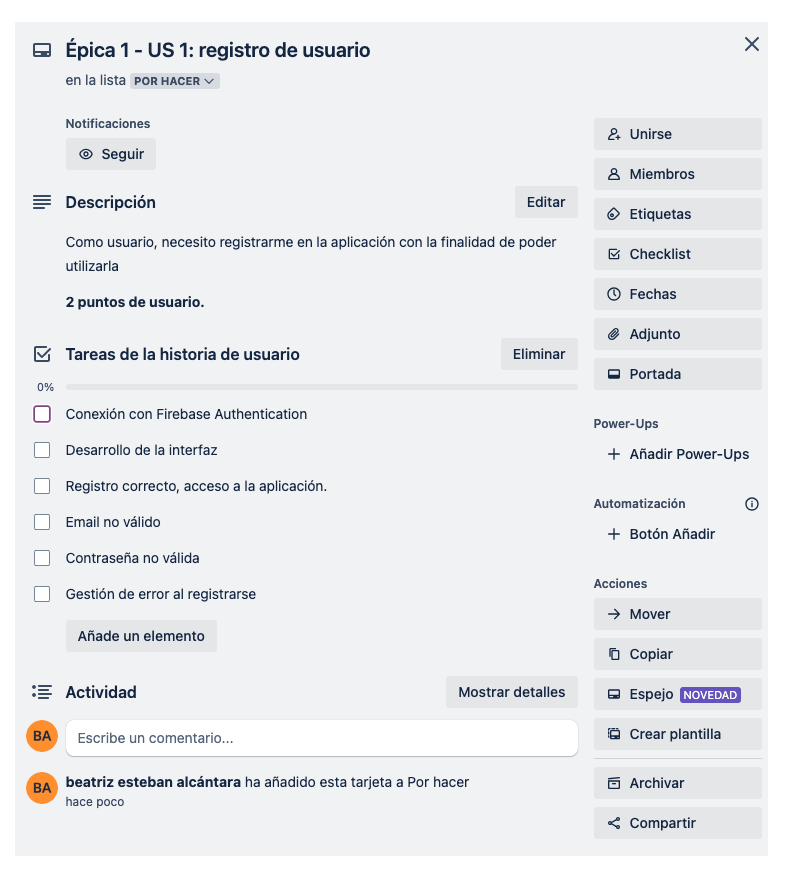
\includegraphics[width=0.6\textwidth]{./img/requirements/user_story_trello.png}
\caption{Historia de usuario en Trello}
\label{fig:user_story_trello}
\end{figure}

\begin{figure}[H]
\centering
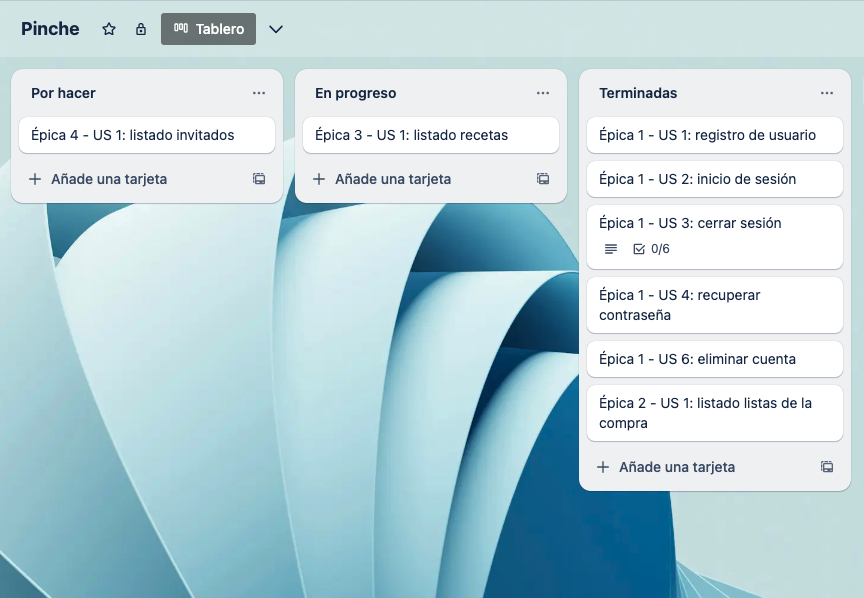
\includegraphics[width=0.6\textwidth]{./img/requirements/final_sprint_trello.png}
\caption{Estado del tablero Kanban al final del primer Sprint}
\label{fig:final_sprint_trello}
\end{figure}

Tras hacer el ejercicio de revisar y reflexionar sobre el Sprint, como marcan la sesión de \textit{Sprint Review} y la de \textit{Sprint Retrospective}, se ajustó el alcance estimado para los siguientes Sprints a un máximo de 8 puntos de historia por iteración, adaptando así la velocidad al contexto real del desarrollo.

Todas las historias de usuario, agrupadas por épica, sus tareas y estimaciones, se adjunta en el anexo \textit{Historias de usuario.xlsx}.

\subsection{Requisitos no funcionales}

Además de la funcionalidad, se han establecido los siguientes requisitos no funcionales:

\begin{itemize}
    \item Conexión con Firestore y creación de repositorios de datos.
    \item Autenticación de usuarios con Firebase Authentication.
    \item Estructura modular y escalable, basada en el patrón arquitectónico MVVM (Model-View-ViewModel).
    \item Inyección de dependecias con Hilt.
    \item Incluir tests tanto unitarios como de interfaz.
\end{itemize}

Estos requisitos definen el alcance funcional y técnico del proyecto, garantizando que el producto final responda tanto a las expectativas del usuario como a criterios de calidad y buenas prácticas del software.

\section{Arquitectura y análisis}
\label{sec:arquitectura-analisis}

La arquitectura de una aplicación móvil resulta de suma importancia para garantizar escalabilidad, optimización del código, rendimiento, solidez, mantenibilidad y la correcta separación de responsabilidades. En este proyecto se ha adoptado la arquitectura recomendada por Android, basada en una estructura en capas y el patrón MVVM (Model-View-ViewModel), con la inclusión de una capa de dominio opcional y la gestión de dependencias mediante Hilt \cite{android-architecture} \cite{mvvm}.

\subsection{Principios generales}

\begin{figure}[H]
\centering
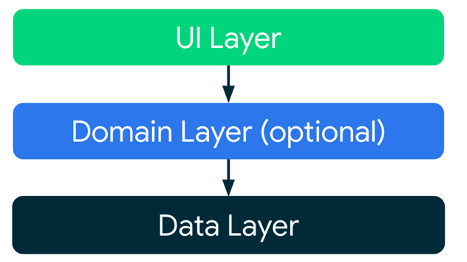
\includegraphics[width=0.6\textwidth]{./img/description/mvvm.png}
\caption{Diagrama arquitectura MVVM. Fuente: \href{https://developer.android.com/topic/architecture?hl=es-419}{Android Developers}}
\label{fig:mvvm}
\end{figure}

Esta arquitectura promueve los principios de separación de responsabilidades, flujo unidireccional de datos, modularidad y testabilidad \cite{android-architecture}. El modelo propuesto divide la lógica de la aplicación en tres capas principales: UI, dominio (opcional) y datos, Figura~\ref{fig:mvvm}. En nuestro caso vamos a utilizar la arquitectura recomendada incluyendo la capa opcional de dominio, Figura~\ref{fig:pinche_architecture}.

\begin{figure}[H]
\centering
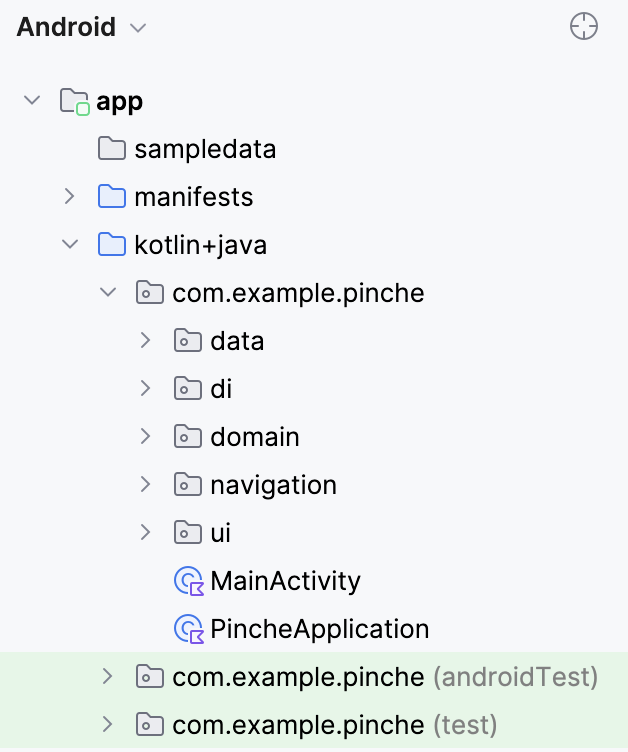
\includegraphics[width=0.6\textwidth]{./img/description/pinche_architecture.png}
\caption{Arquitectura de la aplicación Pinche}
\label{fig:pinche_architecture}
\end{figure}

\subsection{Capa de UI}

La capa de interfaz de usuario es responsable de mostrar los datos al usuario y recoger sus interacciones. Esta capa se compone de dos tipos de elementos:

\begin{itemize}
    \item \textbf{Elementos de la UI}: Son funciones de Jetpack Compose que renderizan los datos en pantalla, Figura~\ref{fig:recoverPasswordView}.
    \item \textbf{Contenedores de estado}: Los ViewModel que retienen el estado de la UI y exponen datos reactivos mediante \textit{StateFlow}, Figura~\ref{fig:recoverPasswordViewModel}.
\end{itemize}

\begin{figure}[H]
\centering
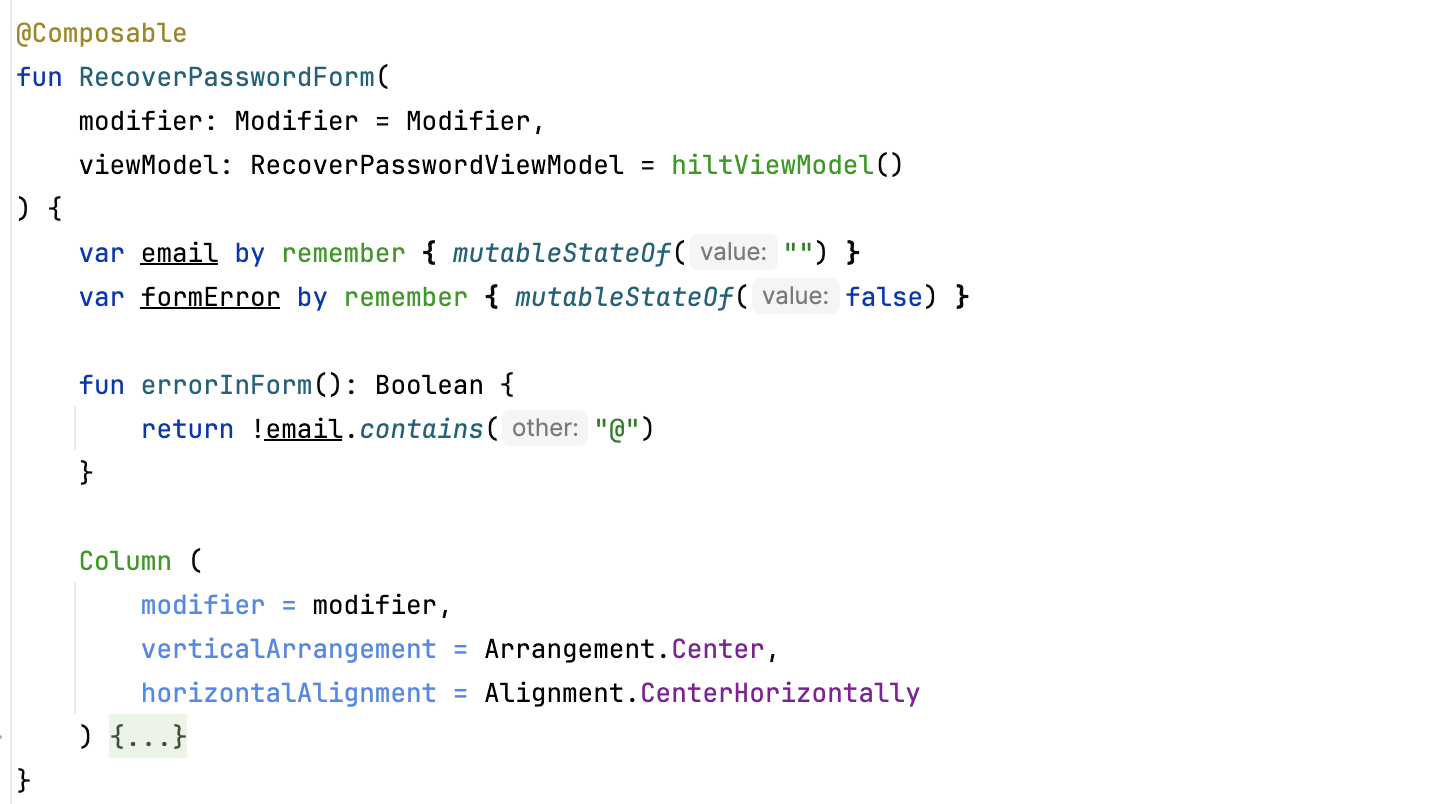
\includegraphics[width=0.7\textwidth]{./img/description/recoverPasswordView.png}
\caption{Componente Compose \textit{RecoverPasswordForm} de Pinche}
\label{fig:recoverPasswordView}
\end{figure}

\begin{figure}[H]
\centering
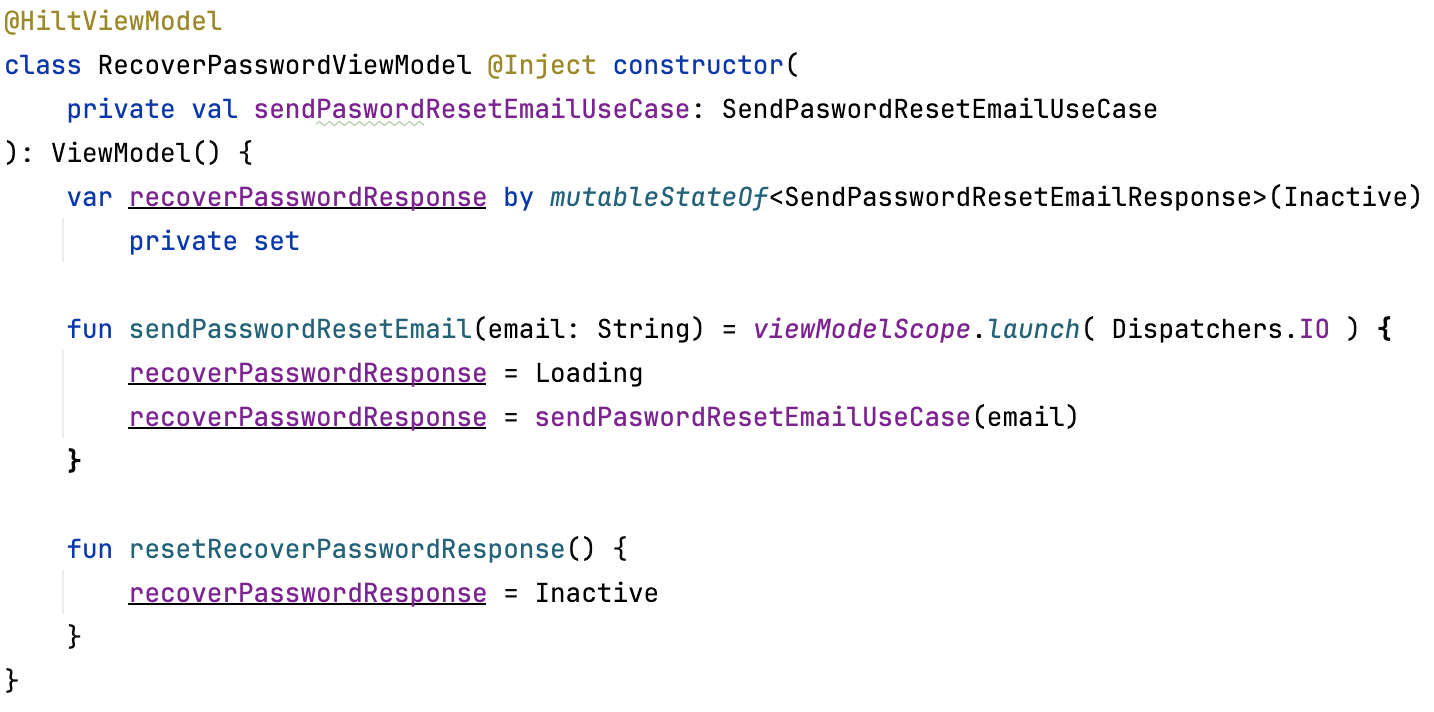
\includegraphics[width=0.7\textwidth]{./img/description/recoverPasswordViewModel.png}
\caption{ViewModel \textit{RecoverPasswordForm} de Pinche}
\label{fig:recoverPasswordViewModel}
\end{figure}

\subsection{Capa de dominio}

La capa de dominio encapsula la lógica empresarial que puede ser compartida entre distintos ViewModels. En ella se definen los casos de uso (\textit{use cases}) como clases que representan acciones o procesos específicos de la aplicación, facilitando la reutilización de código y la claridad del flujo de datos. La Figura~\ref{fig:recoverUseCase} muestra un ejemplo de caso de uso de la aplicación Pinche.

\begin{figure}[H]
\centering
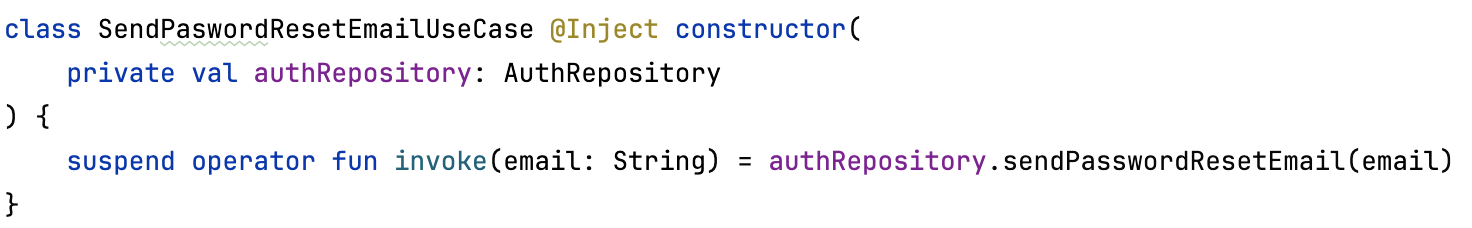
\includegraphics[width=0.7\textwidth]{./img/description/recoverUseCase.png}
\caption{Caso de uso \textit{SendPasswordResetEmailUseCase} de Pinche}
\label{fig:recoverUseCase}
\end{figure}

\subsection{Capa de datos}

Esta capa es responsable de la obtención y persistencia de datos. Se organiza en:

\begin{itemize}
    \item \textbf{Repositorios}: Actúan como intermediarios entre las fuentes de datos y la capa de dominio.
    \item \textbf{Fuentes de datos}: Pueden ser locales o remotas. En nuestro caso, usamos la fuente de datos remota Firebase Authentication que proporciona servicios de autenticación y la base de datos en la nube Firestore \cite{firestore, firebase-auth}.
\end{itemize}

En la Figura~\ref{fig:recoverPassRepo} muestra la función del reposositorio de autenticación responsable de intermediar con Firebase Authentication para recuperar la contraseña de un usuario enviándole un correo electrónico a su dirección de correo.

\begin{figure}[H]
\centering
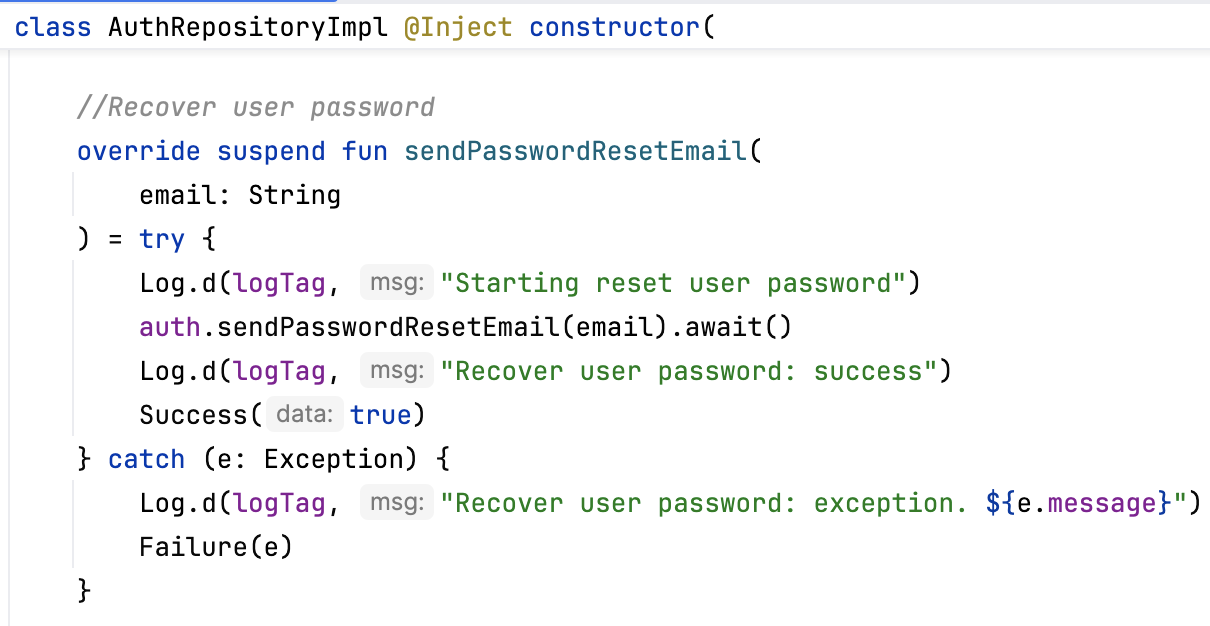
\includegraphics[width=0.7\textwidth]{./img/description/recoverPassRepo.png}
\caption{Función \textit{sendPasswordResetEmail} en el repositorio de autenticación}
\label{fig:recoverPassRepo}
\end{figure}

Gracias a esta separación, si por ejemplo en el futuro se quisiera cambiar de base de datos o el método de autenticación, solo se vería afectada la capa de datos, manteniendo intacto el resto del sistema.

\subsection{Gestión de dependencias con Hilt}

La gestión de dependencias se realiza mediante la biblioteca Hilt como ya hemos comentado. Hilt proporciona objetos preconfigurados a las clases de Android y administra automáticamente su ciclo de vida \cite{hilt}.

Dada la relativa complejidad y el tiempo dedicado a comprender cómo gestiona Hilt las dependecias, considero que merece la pena explicar cómo se ha integrado en Pinche en mayor detalle.

En primer lugar, para que la app Pinche use Hilt debemos usar la anotación \textit{@HiltAndroidApp}para activar la generación de código Hilt, Figura~\ref{fig:pincheAppHilt}.

\begin{figure}[H]
\centering
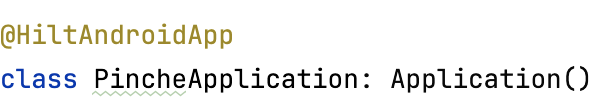
\includegraphics[width=0.7\textwidth]{./img/description/pinche_app_hilt.png}
\caption{Definición de la clase \textit{PincheApplication}}
\label{fig:pincheAppHilt}
\end{figure}

Para realizar una inyección de dependecia, Hilt necesita saber cómo proporcionar una instancia de la misma al componente al que se inyecta. Esto lo realiza a través de vinculaciones, para ello hemos usado inyecciones de constructor a través de la anotación \textit{@Inject} en la construción de la clases de los componentes que necesitan la dependencia. Un ejemplo de inyección de constructor puede verse en el caso de uso \textit{SendPasswordResetEmailUseCase} en la Figura~\ref{fig:recoverUseCase}.

Pero en este caso concreto no sirve unicamente con inyectar \textit{AuthRepository} ya que es una interfaz que se implementa en \textit{AuthRepositoryImpl} y Hilt no permite la insercción de interfaces como dependencia. Para ello necesitamos también generar una vinculación entre la interfaz y la implementación para que Hilt sepa como proporcionar una instancia de la misma. Para ello generamos un módulo de Hilt, con la anotación \textit{@Module} y establecemos el alcance del módulo y de las clases de Android que lo usarán con la anotación \textit{@InstallIn}. La Figura~\ref{fig:authModuleHilt} muestra el modulo de Hilt \textit{AuthModule} con un alcance de toda la aplicación \textit{SingletonComponent::class}. Se necesita también una función abstracta anotada con \textit{@Binds} que concreto que implementación usar para proporcionar una instancia de la interfaz.

\begin{figure}[H]
\centering
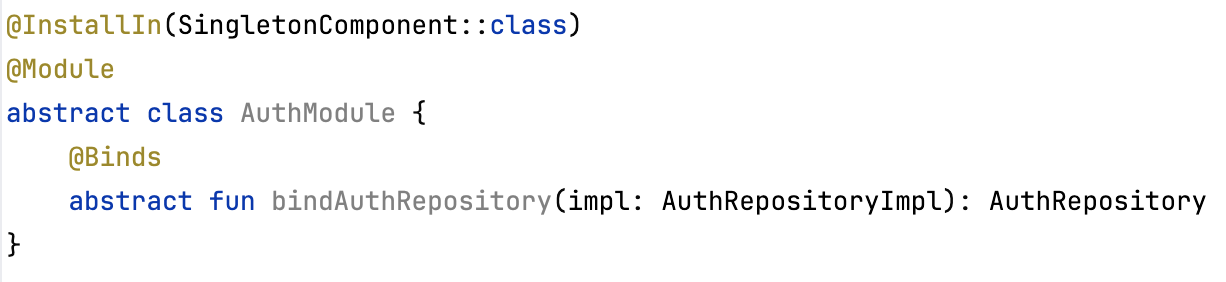
\includegraphics[width=0.7\textwidth]{./img/description/auth_module_hilt.png}
\caption{Módulo Hilt \textit{AuthModule} de Pinche}
\label{fig:authModuleHilt}
\end{figure}

Tampoco se puede inyectar directamente clases que no son de nuestra propiedad y proevienen de bibliotecas externas, como es el caso de Firebase Authentication y Firebase Firestore. Para la insercción de estas clases necesitaremos implementar un módulo Hilt con funciones con la anotación @Provides que indiquen cómo inyectarlas, Figura~\ref{fig:firebaseHilt}.

\begin{figure}[H]
\centering
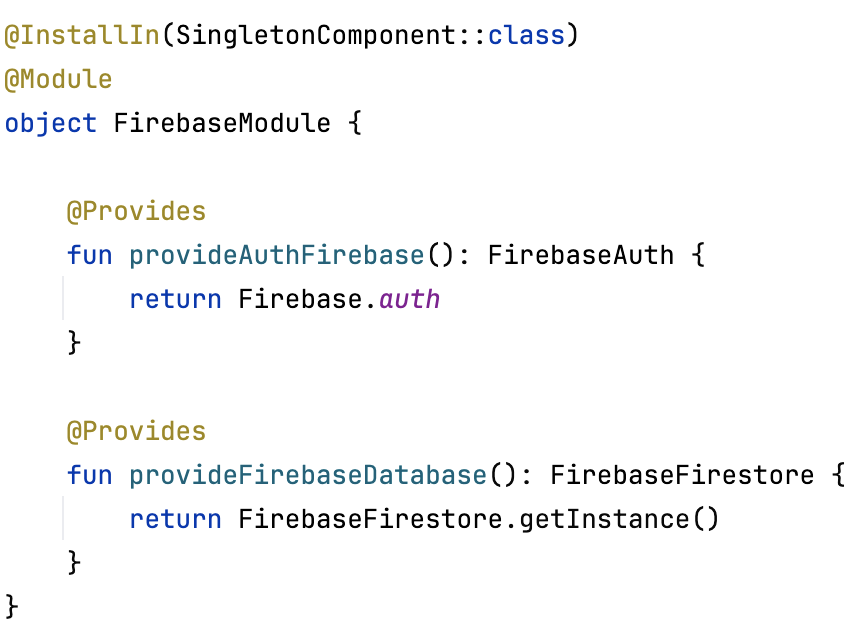
\includegraphics[width=0.7\textwidth]{./img/description/firebase_hilt.png}
\caption{Módulo Hilt \textit{FirebaseModule} de Pinche}
\label{fig:firebaseHilt}
\end{figure}

De esta manera, se consigue que de manera directa y sin pasar las dependencia de un componente a otro, el componente acceda a ella. También veremos en la \autoref{sec:pruebas} lo que facilita sustituir estas dependencias por dependencias simuladas de cara a testear componentes.

\subsection{Ventajas de esta arquitectura}

Esta arquitecura aspectos fundamentales al código de la aplicación Pinche:

\begin{itemize}
    \item Mejor separación de responsabilidades entre componentes.
    \item Mayor facilidad de testeo en todas las capas.
    \item Reutilización de lógica empresarial entre distintas pantallas.
    \item Facilidad para mantener y escalar el código base en el futuro.
\end{itemize}

Este enfoque permite un desarrollo estructurado, coherente y sostenible, favoreciendo además la implementación de buenas prácticas de ingeniería de software.

\section{Diseño e implementación}
\label{sec:diseno-implementacion}

\subsection{Análisis de requerimientos y estructura funcional}

La aplicación ha sido diseñada en base a un conjunto de funcionalidades organizadas en cuatro secciones principales: gestión de cuenta de usuario, listas de la compra, recetas e invitados. Este enfoque permite abordar de forma modular las necesidades de los usuarios y facilita la extensión del sistema.

Para el diseño de la aplicación Pinche utilicé Figma, hice un primer prototipo de cómo iba a organizar y qué estilo iba a seguir. Fue un primer prototipo incompleto, pero que me sirvio para visualizar la aplicación e iterarlo para conseguir una interfaz intuitiva. El salto del diseño a lo realmente implementado es notable, pero la estructura y muchas de las decisiones a las que llegue creando el diseño se han mantenido, Figura~\ref{fig:pincheFigma}.

\begin{figure}[H]
\centering
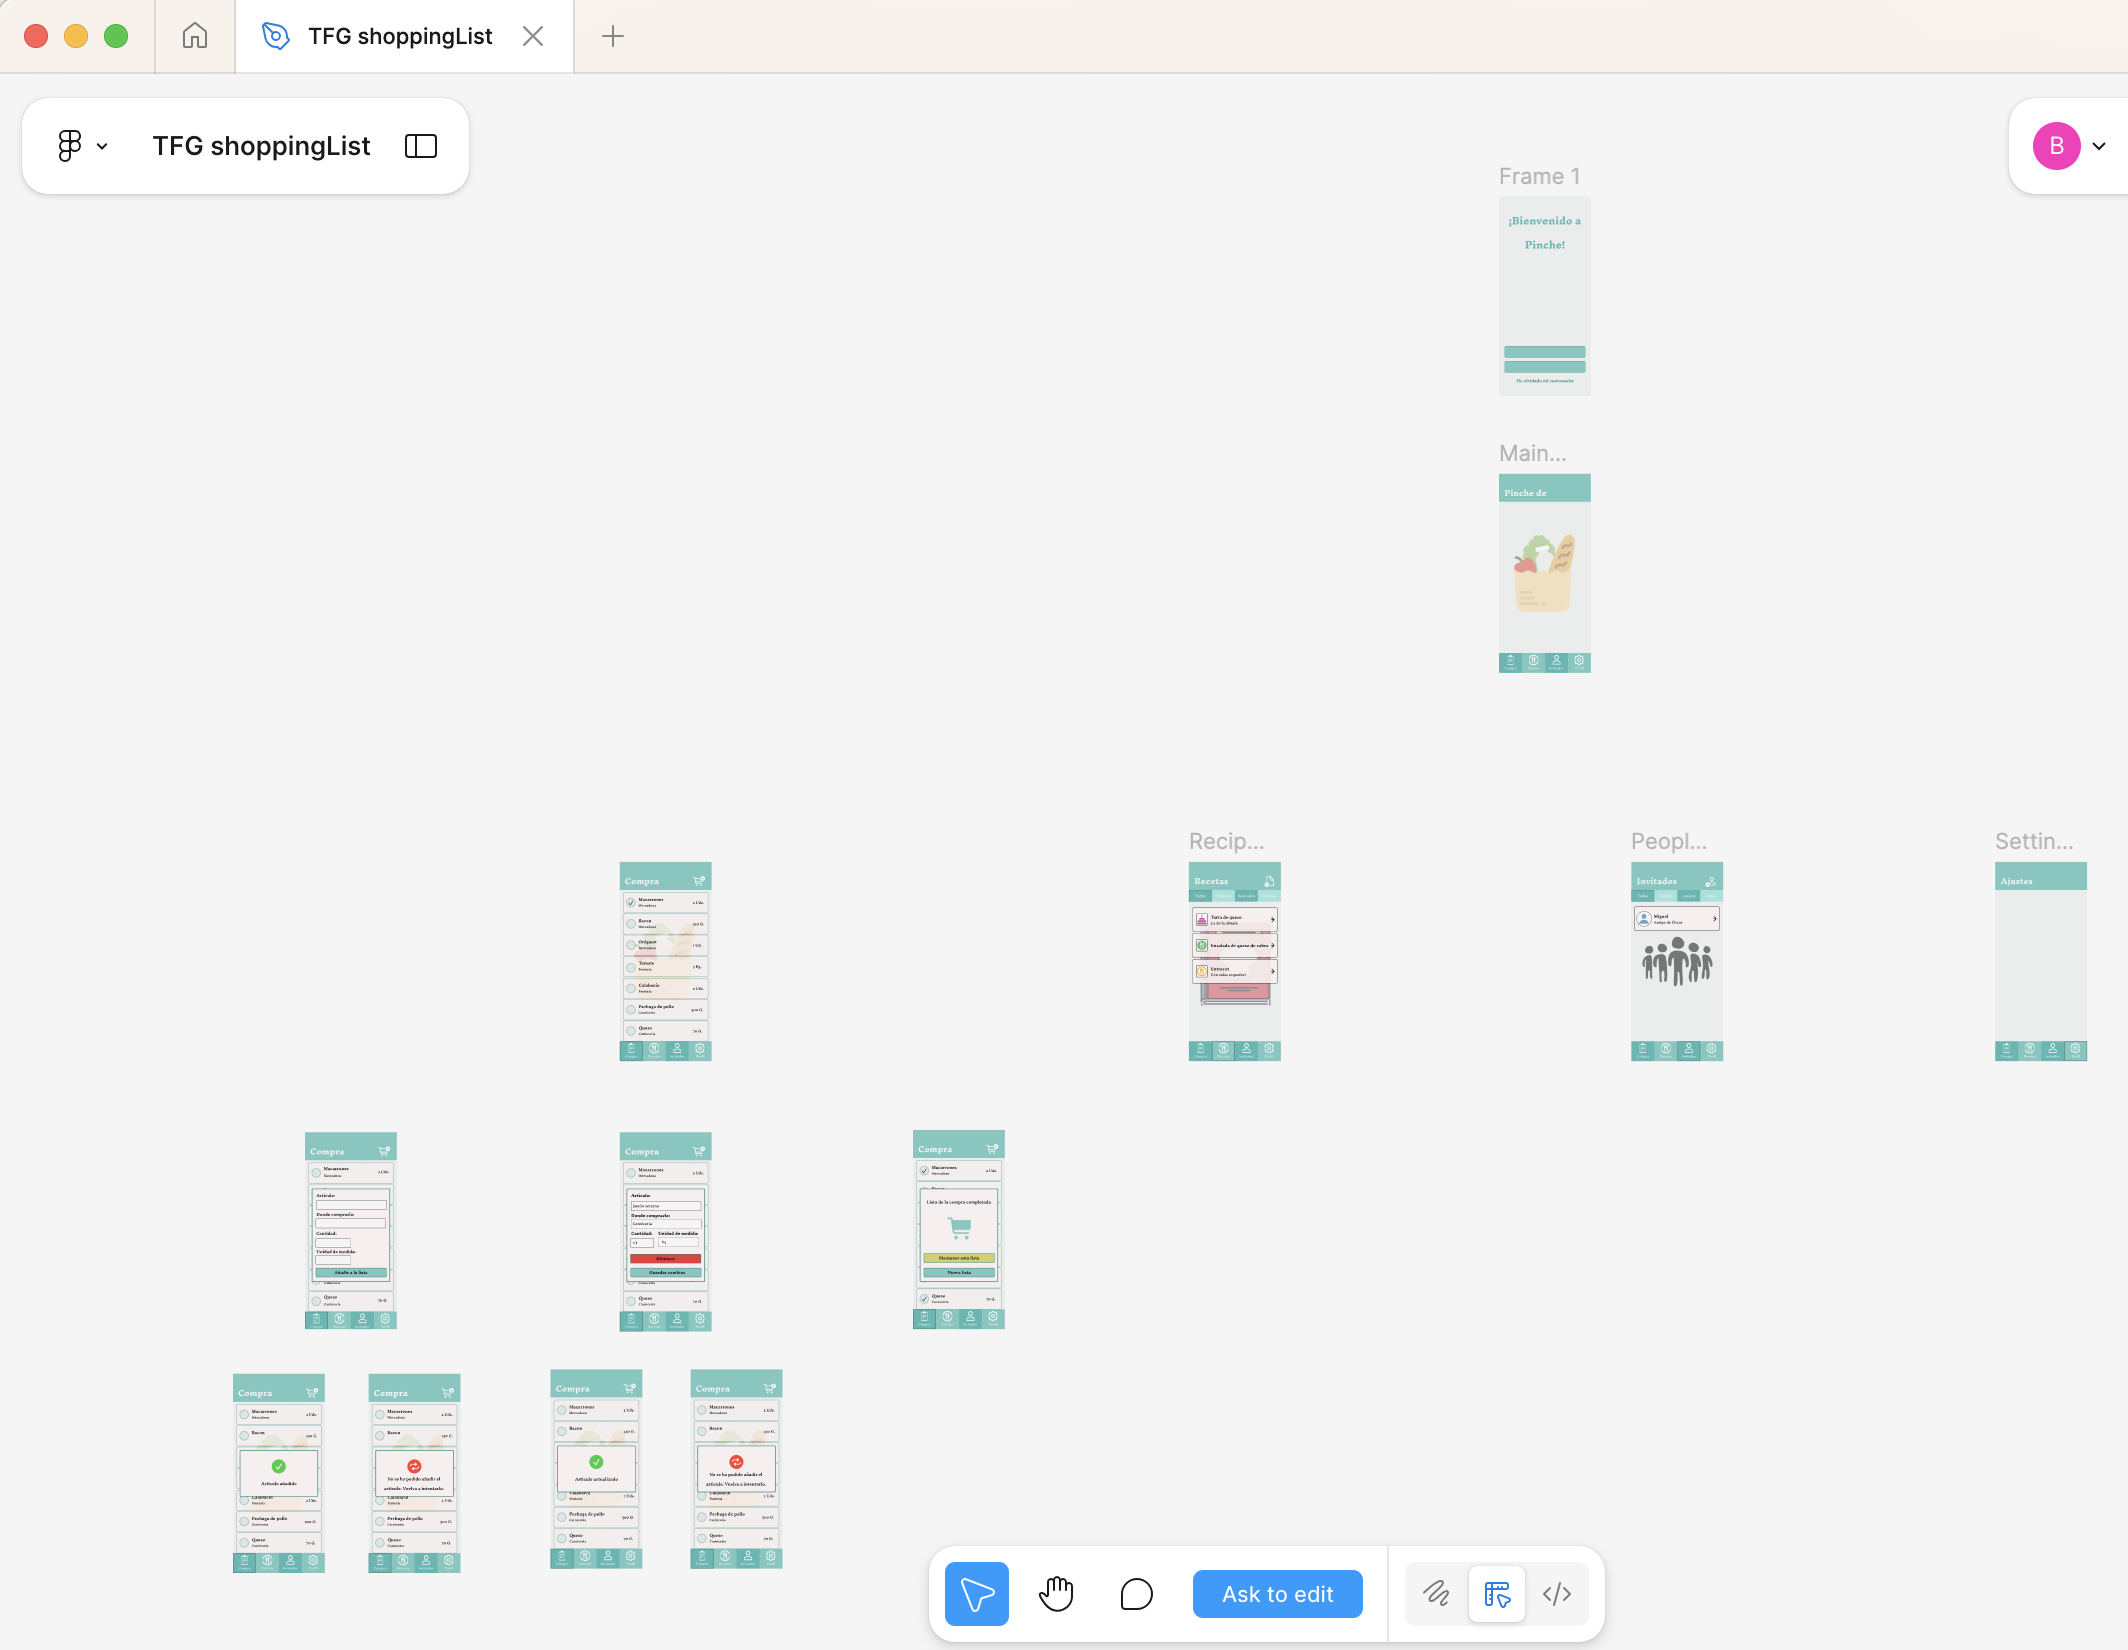
\includegraphics[width=0.9\textwidth]{./img/description/pinche_figma.png}
\caption{Primer prototipo de Pinche en Figma}
\label{fig:pincheFigma}
\end{figure}

\textbf{DIAGRAMAS DE COMPONENTES, DE CASOS DE USO Y ESAS COSAS?}

\textbf{METER CAPTURAS DE LA PROPIA APLICACION.}

El modelo de datos se ha estructurado para cubrir las siguientes entidades principales:

\begin{itemize}
    \item \textbf{Lista}: contiene un conjunto de productos, su nombre y estado.
    \item \textbf{Producto}: asociado a una lista, con nombre, cantidad y supermercado.
    \item \textbf{Receta}: incluye nombre, pasos de elaboración, ingredientes y número de comensales.
    \item \textbf{Ingrediente}: definido por nombre y cantidad relativa a los comensales.
    \item \textbf{Invitado}: con nombre, preferencias alimentarias, intolerancias y registro de comidas anteriores.
\end{itemize}

Este modelo facilita la integración de funcionalidades como el cálculo de ingredientes según el número de comensales, la generación de listas automáticas a partir de recetas y la personalización de menús para invitados con restricciones.


Esta implementación modular y centrada en buenas prácticas garantiza que Pinche pueda mantenerse y escalarse en el tiempo, facilitando la extensi\'on de funcionalidades futuras.

\section{Pruebas}
\label{sec:pruebas}

El asegurar la calidad en el desarrollo de la aplicación Pinche se ha abordado mediante una estrategia de pruebas estructurada que cubre distintos niveles de validación del sistema: pruebas unitarias y de interfaz. Esta estrategia ha permitido verificar que los componentes funcionan correctamente.

\subsection{Pruebas unitarias}

Las pruebas unitarias validan pequeñas unidades de código de forma aislada, como por ejemplo los casos de uso. Para ello se ha utilizado \textbf{JUnit4} como framework base y \textbf{MockK} para simular comportamientos de dependencias externas como repositorios o servicios \cite{android-testing}.

El Listado~\ref{lst:signinTest} muestra la implementación de un test unitario para el caso de uso \textit{SignInUserUseCase} que permite al usuario iniciar sesión en la aplicación.

\begin{lstlisting}[language=Java, caption={SignInUserUseCaseTest}, label={lst:signinTest}]
  @ExperimentalCoroutinesApi
  class SignInUserUseCaseTest {

    @get:Rule
    val coroutinesTestRule = MainDispatcherRule()

    private val authRepository: AuthRepository = mockk()
    private lateinit var signInUserUseCase: SignInUserUseCase

    private val email = "test@email.com"
    private val password = "123456"

    @Before
    fun setup() {
        signInUserUseCase = SignInUserUseCase(authRepository)
    }

    @Test
    fun `sign in returns Success when repository succeeds`() = runTest {
        coEvery { authRepository.firebaseSignInWithEmailAndPassword(email, password) } returns Success(true)

        val result = signInUserUseCase(email, password)

        assertTrue(result is Success)
        coVerify { authRepository.firebaseSignInWithEmailAndPassword(email, password) }
    }

    @Test
    fun `sign in returns Failure when repository fails`() = runTest {
        val exception = Exception("Auth error")
        coEvery { authRepository.firebaseSignInWithEmailAndPassword(email, password) } returns Failure(exception)

        val result = signInUserUseCase(email, password)

        assertTrue(result is Failure)
        coVerify { authRepository.firebaseSignInWithEmailAndPassword(email, password) }
    }
}
\end{lstlisting}

\subsection{Pruebas de interfaz (UI)}

Las pruebas de interfaz de usuario comprueban el estado de las vistas que va a visualizar el usuario como hemos explicado en la \autoref{sec:test-tools}.